% Báo cáo tiến độ 15/10/2026 — cấu trúc assertion–evidence (Garner & Alley 2013):
% tiêu đề mỗi trang là một câu kết luận, thân trang là bằng chứng (hình, biểu đồ).
% Báo cáo tiến độ 15/10/2026 — build: latexmk (XeLaTeX, xem latexmkrc)
\documentclass[aspectratio=169,11pt]{beamer}

\usepackage{fontspec}
\setsansfont{Lato}
\newfontfamily\sym{DejaVu Sans}
\usepackage{booktabs}
\usepackage{array}
\usepackage{tikz}
\usetikzlibrary{arrows.meta,calc,positioning}
\usepackage{pgfplots}
\pgfplotsset{compat=1.18}

% ---------- màu ----------
\definecolor{ink}{HTML}{1F2328}
\definecolor{mute}{HTML}{8A9099}
\definecolor{line}{HTML}{D5DAE1}
\definecolor{accent}{HTML}{2F6FB3}
\definecolor{hot}{HTML}{E07B24}
\definecolor{ok}{HTML}{2E9E5B}

% ---------- giao diện tối giản ----------
\setbeamertemplate{navigation symbols}{}
\setbeamercolor{normal text}{fg=ink,bg=white}
\setbeamercolor{structure}{fg=accent}
\setbeamercolor{frametitle}{fg=ink}
\setbeamercolor{title}{fg=ink}
\setbeamerfont{frametitle}{size=\Large,series=\bfseries}
\setbeamerfont{title}{size=\LARGE,series=\bfseries}
\setbeamertemplate{frametitle}{%
  \vspace*{0.7em}\insertframetitle\par\vspace{0.25em}%
  {\color{accent}\rule{1.2cm}{2pt}}\par}
\setbeamertemplate{footline}{%
  \hfill{\scriptsize\color{mute}\insertframenumber}\hspace*{1.2em}\vspace*{0.8em}}
\setbeamertemplate{itemize item}{\color{accent}\small$\bullet$}
\setbeamertemplate{itemize subitem}{\color{mute}\scriptsize$\bullet$}
\setlength{\parskip}{0pt}

\setbeamertemplate{title page}{%
  \vspace*{1.4cm}
  {\color{accent}\rule{1.5cm}{3pt}}\par\vspace{0.5cm}
  {\usebeamerfont{title}\usebeamercolor[fg]{title}\inserttitle\par}
  \vspace{0.35cm}
  {\large\color{mute}\insertsubtitle\par}
  \vfill
  {\insertauthor\par}\vspace{0.1cm}
  {\small\color{mute}\insertinstitute\quad·\quad\insertdate\par}
  \vspace*{0.9cm}}

\newcommand{\done}{{\sym\color{ok}✓}}
\newcommand{\half}{{\sym\color{hot}◐}}
\newcommand{\todo}{{\sym\color{mute}○}}
\newcommand{\gray}[1]{{\color{mute}#1}}

\title{Học chính sách hành động cộng tác\\người -- robot có nhận thức ý định}
\subtitle{Báo cáo tiến độ}
\author{Đào Duy Hưng}
\institute{GVHD: PGS.TS. Hoàng Văn Xiêm}
\date{15/10/2026}
\newcommand{\ci}[3]{$#1$\,{\color{mute}\scriptsize[$#2$;\,$#3$]}}
\newcommand{\sig}{\textsuperscript{\color{ok}\bfseries*}}

\usepackage{graphicx}

\pgfplotsset{
  bars/.style={ybar, bar width=14pt, ymin=0, ymax=1, axis lines*=left, ymajorgrids, grid style={line},
    tick label style={font=\scriptsize}, label style={font=\scriptsize}, enlarge x limits=0.15,
    nodes near coords, nodes near coords style={font=\scriptsize, color=ink},
    /pgf/number format/fixed, /pgf/number format/precision=2}}

\begin{document}

% =====================================================================
\begin{frame}[plain]
  \titlepage
\end{frame}

% =====================================================================
\begin{frame}{Đề tài hỏi: biết ý định của người có giúp robot hành động sớm hiệu quả hơn không?}
  \begin{columns}[c]
    \begin{column}{0.52\textwidth}
      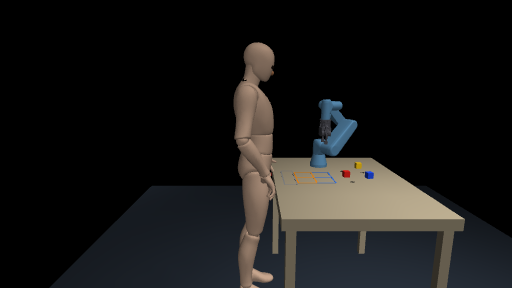
\includegraphics[width=\linewidth]{figures/scene_side.png}

      \scriptsize\gray{Ví dụ (task T1): trên bàn có hai khối đỏ giống hệt. Chỉ cử chỉ chỉ tay của người cho biết lấy khối nào.}
    \end{column}
    \begin{column}{0.45\textwidth}
      \small
      Thiết kế 2$\times$2: bốn robot học từ demo, khác nhau ở hai điểm.

      \vspace{0.5em}
      \centering
      \begin{tabular}{@{}lcc@{}}
        \toprule
        & \multicolumn{2}{c}{Robot có nhận ý định?} \\
        \cmidrule(l){2-3}
        Demo hành động & Không & Có \\
        \midrule
        Trễ (chờ người làm xong) & A & C \\
        Sớm (đoán khi đang làm) & B & D \\
        \bottomrule
      \end{tabular}

      \vspace{0.6em}
      \raggedright
      \textbf{Giả thuyết:} D tốt hơn B nhiều hơn mức C tốt hơn A, tức là ý định có ích nhất khi hành động sớm.
    \end{column}
  \end{columns}
\end{frame}

% =====================================================================
\begin{frame}{Hệ thống: bộ đo đọc cử chỉ thành ý định, robot học hành động từ ảnh và ý định}
  \centering
  \begin{tikzpicture}[
      box/.style={draw=line, rounded corners=3pt, minimum height=1.1cm, align=center, font=\small, inner sep=5pt},
      key/.style={box, draw=accent, fill=accent!8, line width=0.9pt},
      arr/.style={-{Stealth[length=5pt]}, color=mute, line width=0.8pt}]
    \node[box, minimum width=2.3cm] (h) at (0,0) {Người\\\scriptsize chỉ tay, chìa tay, vươn tay};
    \node[box, minimum width=2.7cm] (dp) at (4.7,1.0) {Bộ đo ý định (robot C, D)\\\scriptsize DeePoint: xác suất từng đích};
    \node[box, minimum width=2.7cm] (cam) at (4.7,-1.0) {Camera\\\scriptsize và trạng thái robot};
    \node[key, minimum width=2.6cm] (act) at (8.7,0) {Policy ACT\\\scriptsize học bắt chước};
    \node[box, minimum width=2.2cm] (rb) at (12.0,0) {Robot\\\scriptsize hành động 2 s tới};
    \draw[arr] (h.east) -- ++(0.7,0) |- (dp.west);
    \draw[arr] (h.east) -- ++(0.7,0) |- (cam.west);
    \draw[arr] (dp.east) -- ++(0.4,0) |- ([yshift=4pt]act.west);
    \draw[arr] (cam.east) -- ++(0.4,0) |- ([yshift=-4pt]act.west);
    \draw[arr] (act.east) -- (rb.west);
  \end{tikzpicture}

  \vspace{1em}
  \small
  \begin{tabular}{@{}l>{\raggedright\arraybackslash}p{0.7\linewidth}@{}}
    \toprule
    Demo sớm & robot bắt đầu làm khi bộ đo tin $\geq 70\%$ vào một đích, lúc người còn đang làm cử chỉ \\
    Demo trễ & robot chờ người làm xong cử chỉ và bộ đo tin $\geq 95\%$ \\
    \bottomrule
  \end{tabular}
\end{frame}

% =====================================================================
\begin{frame}{Đo bằng hai chỉ số chuẩn: robot có làm xong việc, và chọn đúng đích lúc nào}
  \centering
  \begin{tikzpicture}[font=\small]
    \draw[line, line width=1pt, -{Stealth[length=5pt]}] (0,0) -- (11,0) node[right, text=mute, font=\scriptsize] {thời gian};
    \fill[accent!15] (1.5,-0.25) rectangle (5.5,0.25);
    \node[font=\scriptsize, text=accent] at (3.0,0.55) {người làm cử chỉ};
    \draw[accent, line width=1pt] (5.5,-0.4) -- (5.5,0.4);
    \node[font=\scriptsize] at (5.5,-0.75) {cử chỉ xong};
    \draw[ok, line width=1pt] (4.2,-0.4) -- (4.2,0.4);
    \node[font=\scriptsize, text=ok, align=center] at (3.5,-0.95) {robot chọn\\đúng đích};
    \draw[hot, line width=1pt] (8.5,-0.4) -- (8.5,0.4);
    \node[font=\scriptsize, text=hot, align=center] at (8.5,-0.95) {robot chọn\\đúng đích};
    \draw[{Stealth[length=4pt]}-{Stealth[length=4pt]}, ok] (4.2,1.1) -- (5.5,1.1) node[midway, above, font=\scriptsize] {AM $> 0$};
    \draw[{Stealth[length=4pt]}-{Stealth[length=4pt]}, hot] (5.5,1.1) -- (8.5,1.1) node[midway, above, font=\scriptsize] {AM $< 0$};
  \end{tikzpicture}

  \vspace{1.2em}
  \small
  \begin{tabular}{@{}l>{\raggedright\arraybackslash}p{0.66\linewidth}l@{}}
    \toprule
    Chỉ số & Nghĩa & Tốt khi \\
    \midrule
    CSR & tỉ lệ episode robot làm xong task & cao \\
    AM (giây) & robot chọn đúng đích sớm hơn lúc người làm xong cử chỉ bao nhiêu ($>0$: đoán trước, $<0$: chọn sau) & cao \\
    \bottomrule
  \end{tabular}

  \vspace{0.5em}
  \scriptsize\gray{Chỉ số theo bộ đánh giá HRIBench. Mọi so sánh chạy trên cùng các episode chưa dùng để huấn luyện.}
\end{frame}

% =====================================================================
\begin{frame}{Học từ demo sớm giúp robot chọn đúng đích sớm hơn khoảng 1--1.5 giây}
  \centering
  \begin{tikzpicture}
    \begin{axis}[xbar, bar width=9pt, width=10.5cm, height=5.6cm, xmin=-4.6, xmax=0,
        axis lines*=left, xmajorgrids, grid style={line},
        symbolic y coords={A: trễ,C: trễ + ý định,expert trễ,B: sớm,D: sớm + ý định,expert sớm},
        ytick=data, y dir=reverse, tick label style={font=\scriptsize}, label style={font=\scriptsize},
        xlabel={AM: thời điểm chọn đúng đích so với lúc cử chỉ xong (giây; gần 0 là sớm hơn)},
        nodes near coords, nodes near coords style={font=\scriptsize, color=ink},
        /pgf/number format/fixed, /pgf/number format/precision=1]
      \addplot[fill=mute!40, draw=mute] coordinates {(-4.03,A: trễ) (-3.14,C: trễ + ý định) (-2.98,expert trễ)};
      \addplot[fill=accent!60, draw=accent] coordinates {(-3.22,B: sớm) (-2.33,D: sớm + ý định) (-1.34,expert sớm)};
    \end{axis}
  \end{tikzpicture}

  \vspace{0.3em}
  \small Robot học từ demo sớm (B, D) chọn đích sớm hơn robot học từ demo trễ (A, C).
  D so với A: \ci{+1.80}{+0.27}{+3.98} giây, có ý nghĩa thống kê.
\end{frame}

% =====================================================================
\begin{frame}{Nhưng robot D ban đầu không dùng ý định: che ý định đi, kết quả không đổi}
  \begin{columns}[c]
    \begin{column}{0.46\textwidth}
      \centering
      \begin{tikzpicture}
        \begin{axis}[bars, width=6.0cm, height=5.2cm, symbolic x coords={có ý định,che ý định}, xtick=data,
            ylabel={CSR (T1--T3, 24 episode)}]
          \addplot[fill=mute!40, draw=mute] coordinates {(có ý định,0.42) (che ý định,0.42)};
        \end{axis}
      \end{tikzpicture}
    \end{column}
    \begin{column}{0.52\textwidth}
      \small
      \textbf{Nguyên nhân tìm được:} trong dữ liệu đưa vào mạng, phần cho biết ``vật nào'' nhỏ hơn các phần khác 20--40 lần, nên mạng không nhìn thấy nó.

      \vspace{0.6em}
      \textbf{Đã kiểm tra và loại trừ:}
      \begin{itemize}
        \item ý định và hành động bị lệch thời gian;
        \item ý định mâu thuẫn với hành động của expert.
      \end{itemize}

      \vspace{0.4em}
      Vậy lợi thế AM của D ở trang trước đến từ demo sớm, chưa phải từ ý định.
    \end{column}
  \end{columns}
\end{frame}

% =====================================================================
\begin{frame}{Sau khi sửa cách mã hoá, robot dùng ý định: ý định sai làm robot làm sai nhiều hơn}
  \begin{columns}[c]
    \begin{column}{0.5\textwidth}
      \centering
      \begin{tikzpicture}
        \begin{axis}[bars, width=6.6cm, height=5.4cm,
            symbolic x coords={có ý định,che ý định,ý định bị hoán}, xtick=data,
            ylabel={CSR của D sau sửa (T1--T3, 24 episode)}]
          \addplot[fill=accent!60, draw=accent] coordinates {(có ý định,0.46) (che ý định,0.33) (ý định bị hoán,0.17)};
        \end{axis}
      \end{tikzpicture}
    \end{column}
    \begin{column}{0.48\textwidth}
      \small
      \textbf{Ý định bị hoán:} giữ nguyên cảnh, nhưng đưa cho robot ý định chỉ sang vật sinh đôi.

      \vspace{0.6em}
      \scriptsize
      \begin{tabular}{@{}lc@{}}
        \toprule
        So sánh ghép cặp & Chênh \\
        \midrule
        CSR: có so với che & \ci{+0.13}{+0.03}{+0.25} \\
        AM: có so với che (s) & \ci{+0.78}{+0.03}{+1.89} \\
        Chọn đúng vật: hoán so với có & \ci{-0.28}{-0.44}{-0.13} \\
        \bottomrule
      \end{tabular}

      \vspace{0.5em}
      Khi ý định trái với điều nhìn thấy, robot \textbf{do dự} chứ không lấy nhầm vật.
    \end{column}
  \end{columns}
\end{frame}

% =====================================================================
\begin{frame}{So với robot không có ý định (B), robot D chưa tốt hơn rõ rệt}
  \centering
  \begin{tikzpicture}
    \begin{axis}[bars, width=11cm, height=5.3cm, bar width=16pt,
        symbolic x coords={A,C,B,D,D sau sửa,expert trễ,expert sớm}, xtick=data,
        xticklabels={A,C,B,D,{D sau\\sửa},{expert\\trễ},{expert\\sớm}}, xticklabel style={align=center},
        ylabel={CSR, task có ý định (32 episode)},
        nodes near coords style={font=\scriptsize, color=ink, anchor=south west, xshift=1pt}]
      \addplot[fill=accent!60, draw=accent, error bars/.cd, y dir=both, y explicit, error bar style={color=mute}] coordinates {
        (A,0.25) -= (0,0.12) += (0,0.17)
        (C,0.19) -= (0,0.10) += (0,0.16)
        (B,0.34) -= (0,0.14) += (0,0.18)
        (D,0.34) -= (0,0.14) += (0,0.18)
        (D sau sửa,0.38) -= (0,0.15) += (0,0.17)
        (expert trễ,0.84) -= (0,0.16) += (0,0.09)
        (expert sớm,0.88) -= (0,0.16) += (0,0.07)};
    \end{axis}
  \end{tikzpicture}

  \small D sau sửa so với B (ghép cặp): CSR \ci{+0.03}{-0.16}{+0.22}. Thanh dọc là khoảng tin cậy 95\%: 32 episode chỉ đủ phát hiện chênh lớn ($\geq 0.20$). Mọi robot còn kém expert xa, chủ yếu do lỗi thao tác (va vật, hết giờ).
\end{frame}

% =====================================================================
\begin{frame}{Câu hỏi nghiên cứu: một phần đã có câu trả lời, câu hỏi chính còn mở}
  \centering\small
  \begin{tabular}{@{}cl>{\raggedright\arraybackslash}p{0.5\linewidth}@{}}
    \toprule
    & Câu hỏi & Bằng chứng hiện có \\
    \midrule
    \done & Robot học được hành động sớm? (A vs B) & Có: chọn đích sớm hơn 1--1.5 s \\
    \done & Robot có dùng được ý định? & Có, sau khi sửa: che hay hoán ý định đều làm kết quả kém đi \\
    \half & Ý định giúp khi hành động sớm? (B vs D) & Có lợi so với chính D khi che ý định; chưa vượt B \\
    \todo & Ý định giúp khi hành động trễ? (A vs C) & Chưa phân định \\
    \todo & Ý định có ích nhất khi sớm? (tương tác) & Chưa phân định; cần khoảng 96 cặp episode \\
    \bottomrule
  \end{tabular}

  \vspace{0.6em}
  \gray{\done{} đã trả lời \quad \half{} trả lời một phần \quad \todo{} chưa trả lời}
\end{frame}

% =====================================================================
\begin{frame}{Đóng góp: phương pháp và phát hiện đã có, kiểm định giả thuyết chính còn sơ bộ}
  \centering\small
  \begin{tabular}{@{}>{\raggedright\arraybackslash}p{0.52\linewidth}ll@{}}
    \toprule
    Đóng góp & Loại & Mức độ \\
    \midrule
    Khung thí nghiệm 2$\times$2 tách ``hành động sớm'' khỏi ``có ý định'' trong học bắt chước & định lượng & \done{} đã xây \\
    Phép kiểm chứng robot có thật sự dùng ý định (che, hoán ý định) & định lượng & \done{} có kết quả \\
    Phát hiện: cách mã hoá làm mạng bỏ qua ý định, và cách sửa & định lượng & \done{} có kết quả \\
    Kiểm định ``ý định giúp hành động sớm'' & định lượng & \half{} sơ bộ \\
    \bottomrule
  \end{tabular}

  \vspace{0.6em}
  \raggedright
  Kết quả chủ yếu \textbf{định lượng} (chỉ số chuẩn, so sánh ghép cặp, khoảng tin cậy 95\%). \textbf{Định tính} chỉ để minh hoạ (video, mô tả hành vi như robot do dự).
\end{frame}

% =====================================================================
\begin{frame}{Tiếp theo: kiểm định giả thuyết chính với đủ dữ liệu, và xin ý kiến thầy}
  \begin{columns}[T]
    \begin{column}{0.48\textwidth}
      \small\textbf{Kế hoạch}
      \begin{itemize}
        \item Tăng số episode đánh giá, đủ để phát hiện chênh có ý nghĩa thực tế.
        \item So B và D khi có ít demo (5 / 10 / 20 mỗi task): ý định có giúp học nhanh hơn không.
        \item Bộ đo đã biết đúng vật sau khoảng 0.75 s; cần robot dùng thông tin này sớm hơn.
      \end{itemize}
    \end{column}
    \begin{column}{0.48\textwidth}
      \small\textbf{Xin ý kiến thầy}
      \begin{enumerate}
        \item Nên kiểm định ở cùng lượng dữ liệu, hay theo hướng ``ít dữ liệu hơn''?
        \item Chênh bao nhiêu là có ý nghĩa thực tế (ví dụ +0.10 hay +0.15 CSR)?
        \item Ngưỡng hành động sớm 70\% đôi khi chọn nhầm lúc đầu: giữ cố định hay đặt theo tỉ lệ nhầm cho phép?
      \end{enumerate}
    \end{column}
  \end{columns}
\end{frame}

\end{document}
